\documentclass[11pt]{article}
\usepackage[margin=0.5in, top=0.2in]{geometry}
\usepackage[all]{nowidow}
\usepackage[hyperfigures=true, hidelinks, pdfhighlight=/N]{hyperref}
\usepackage[separate-uncertainty=true, group-digits=false]{siunitx}
\usepackage{graphicx,amsmath,physics,tabto,float,amssymb,pgfplots,verbatim,tcolorbox}
\usepackage{listings,xcolor,subfig,caption,import,wrapfig}
\usepackage[version=4]{mhchem}
\usepackage[noabbrev]{cleveref}
\newcommand{\creflastconjunction}{, and\nobreakspace}
\definecolor{stringcolor}{HTML}{C792EA}
\definecolor{codeblue}{HTML}{2162DB}
\definecolor{commentcolor}{HTML}{4A6E46}
\captionsetup{font=small, belowskip=0pt}
\renewcommand{\lstlistingname}{Appendix}
\pgfplotsset{compat=1.17}

\begin{document}

\begin{enumerate}
    \setcounter{enumi}{3}
    \item We begin by considering the Schr\"odinger equation for the harmonic oscillator:
    \begin{equation}
        -\frac{\hbar^2}{2m}\frac{d^2\psi}{dx^2}+\frac{m\omega^2x^2}{2}\psi=E\psi
    \end{equation}
    Firstly, to make some things easier, we will consider the values of $\hbar$, $\omega$, and $m$ to be 1. Now in order to approximate the second derivative in the equation above, we will use a finite difference scheme, namely a second order, centred difference. To do this, we first need to create a grid of $x$ points, which we will consider on the interval $[-5,5]$ with 1000 grid points $x_i$. We will use the notation $\psi(x_i)=\psi_i$. Now we can discuss the approximation of the derivative:
    \begin{equation}
        \frac{d^2\psi}{dx^2}\approx\frac{\psi_{i-1}-2\psi_i+\psi{i+1}}{\Delta x^2}
    \end{equation}
    where $\Delta x$ is 10/1000, the distance between grid points.

    Now we can rewrite our Schr\"odinger equation in its discretised form:
    \begin{equation}
        -\frac{1}{2}\frac{\psi_{i-1}-2\psi_i+\psi{i+1}}{\Delta x^2}+\frac{x^2}{2}\psi_i=E\psi_i
    \end{equation}
    We can simply inspect the equation to find the matrix that can act on $\psi$ to give us $E\psi$, finding it to be 
    \begin{equation}
        H=
        \begin{pmatrix}
            \frac{1}{\Delta x^2}+\frac{x^2}{2} & -\frac{1}{2\Delta x^2} & 0 & \dots & 0 \\
            -\frac{1}{2\Delta x^2} & \frac{1}{\Delta x^2}+\frac{x^2}{2} & -\frac{1}{2\Delta x^2} & \dots & 0 \\
            \vdots & \ddots & \ddots & \ddots & \vdots \\
            0 & \dots & -\frac{1}{2\Delta x^2} & \frac{1}{\Delta x^2}+\frac{x^2}{2} & -\frac{1}{2\Delta x^2} \\
            0 & \dots & 0 & -\frac{1}{2\Delta x^2} & \frac{1}{\Delta x^2}+\frac{x^2}{2} \\
        \end{pmatrix}
    \end{equation}
    We can use any method to solve this system for its eigenvalues and eigenvectors, and we chose to use the \texttt{Eigensystem} method from Mathematica. This method spits out all $N$ eigenvalues and eigenvectors, for $N$ being the size of the matrix, in our case 1000, so we simply chose the last 4, which were
    
    \begin{table}[H]
        \centering
        \begin{tabular}{c c c c}
            $E=$ 0.499997 & 1.49998 & 2.49996 & 3.49992
        \end{tabular}
    \end{table}

    This is fairly close to the expected $0.5, 1.5, 2.5, 3.5$, in units of $\hbar\omega$ of course, and can be improved by increasing the number of grid points. The corresponding eigenvectors were
    \begin{figure}[h]
        \begin{center}
            \scalebox{0.5}{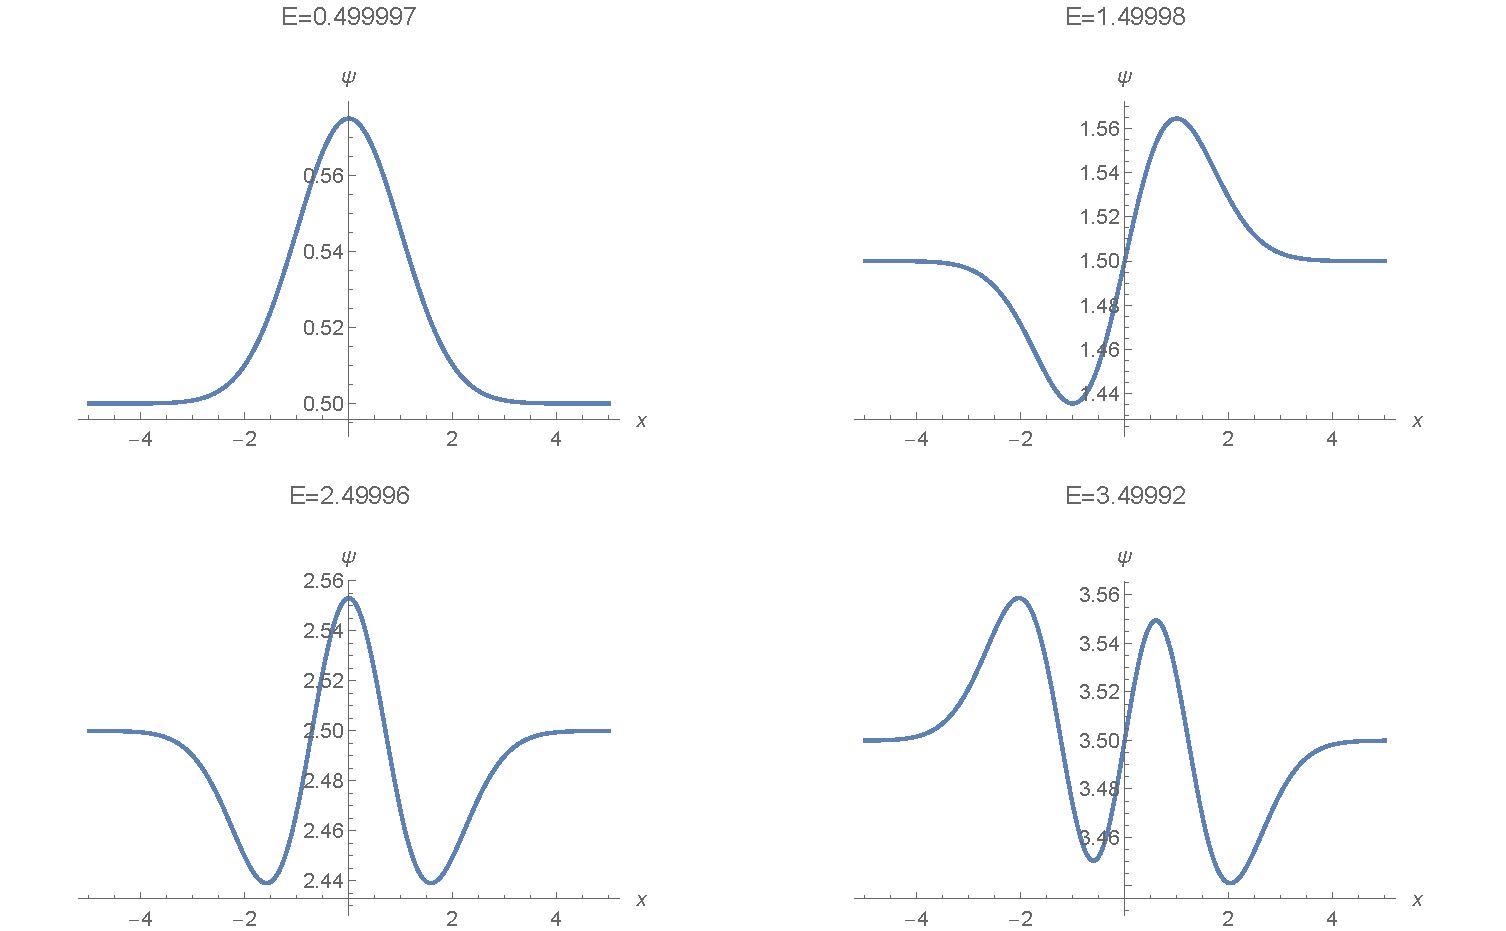
\includegraphics{Q4_plots.pdf}}
        \end{center}
    \end{figure}
    


\end{enumerate}

\end{document}